\documentclass{article}
\usepackage{multicol}
\usepackage{titlesec}
\usepackage[margin=0.75in]{geometry}
\usepackage{pgfplots}
% MACROS %

\titleformat{\section}
  {\large\scshape\filcenter}{\thesection}{}{}

\begin{document}

\title{\textbf{Optimal Scheduling of Introductory Programming Lab}}
\author{
   Chris Alfino \textit{\&} Rajan Selvan\\
   \vspace{12pt}
   \small\textit{Math 480}\\
   Connor Moore\\
   \small\textit{CSE TA Coordinator}}
\date{}

\maketitle
\noindent\makebox[\linewidth]{\rule{\textwidth}{0.4pt}}

\setlength\columnsep{0.45in}
\setlength{\parskip}{0.5em}
\begin{multicols}{2}

\section*{Background}

In recent years, enrollment in the University of Washington's introductory computer science classes, CSE 142 and CSE 143, has skyrocketed. Students are interested in programming for a variety of reasons; industry and academic research positions abound, while programming skills are becoming increasingly necessary in other disciplines around campus. In Winter 2014, CSE 142 and 143 each hit new enrollment records: 810 and 530 students respectively! In order to meet new demand, CSE 142 and 143 have needed to scale their educational efforts. Requisite hiring of undergraduate teaching assistants has increased in proportion with enrollment, with each TA-lead discussion section containing roughly 20 students.

The introductory programming lab (IPL) in Mary Gates Hall is a two room computer lab open from 12:30pm to 9:30pm every week day and from 1:30pm to 3:30pm on Saturday and Sunday. Students in CSE 142 and 143 can come to the lab during these hours to be helped with conceptual and homework questions by whichever TAs are currently staffed. A queuing system in the lab allows a student to add him/herself to a help queue through a web interface. The process for a working TA is then straightforward: he/she dequeues a student and helps the student one-on-one for 2 to 10 minutes. A TA typically signs up for 2 one-hour schedule slots each week, so that the number of TAs in the lab ranges from as few as 1 or 2 on weekends to as many as 7 on busy weekday evenings.

As it stands, the CSE department's approach to IPL staffing is not scalable. At a meeting with all sixty-seven TAs in attendance, the TA coordinator put the entire IPL schedule up on a projector screen, and proceed to call on each TA in order from most to least senior. Each TA responds with his/her top choice among time slots not taken, and the TA coordinator tentatively schedules that choice. Toward the end of the process, when younger TAs are predictably choosing from among the least popular time slots, conflicts inevitably arise. Resolution usually requires that TAs volunteer to swap assignments, and coordinators negotiate the schedule switches in real time. The approach is ultimately effective, but fails to capture more nuanced TA preferences and becomes increasingly unmanageable with large TA numbers.

\section*{Objective}

At a high level, \textit{our goal was to schedule TA IPL shifts such that minimum and maximum staffing requirements are met and TA preferences are accommodated as much as possible}. The CSE department has a number of easily formalized requirements for staffing, including minimum numbers of total and senior TAs required for each time slot. A \textit{senior TA} is a TA that has instructed for at least three quarters. For our main problem, we assumed that the departments quotas for TAs at each time slot were set in stone.

TAs have some preferences that cannot be ignored in scheduling hours. Each student has hours that they cannot work (during class, for instance), and also preferences about when they'd like to work. As a goal, we would like to maximize TA preference accommodation, splitting ties according to TA seniority (number of quarters taught). These preferences must be balanced, however, with the need to compose groups of ideally mixed seniority during key hours. Before a particularly tough CSE 143 assignment, it is essential that more experienced TAs are present to field questions and help less experienced TAs. These factors are weighed into the objective function in a way that is customizable in the future.

As a stretch goal, we sought to provide a simulation tool to model IPL queue behavior with the hope that such a tool would provide a way to evaluate different sets of staffing requirements. A good set of quotas minimizes queue response time, but the problem is complicated by various factors: how much does the presence of senior TAs affect service time? what is the best dequeuing policy when faced with 2-minute and 10-minute queues that are both full? The CS department has already done some work to accommodate varying student demand across the week. More students arrive at the IPL during the hours before important due dates for instance, so more TAs are staffed during these hours. Over the past couple years, data has been collected about the frequency of CSE 142 and 143 student questions at various times of the day.

\section*{Basic LP}
Our problem can be formulated as a general assignment problem, with $m$ TAs and $n$ time slots. Under this formulation, we let $x_{ij}$ be a 0-1 variable where $x_{ij} = 1$ if TA $i$ works time slot $j$ and $x_{ij} = 0$ otherwise.

For each TA $i$, let $s_i = 1$ if TA $i$ is a senior TA, 0 otherwise. Each TA must work at least two hours each week and can work up to a self-imposed maximum $m_i$ hours. As undergraduate UW employees, TAs cannot legally work more than 19.5 hours. Formally for each TA $i$,

\begin{equation}
2 \leq \sum_{j=1}^{n}x_{ij} \leq \textrm{min}(m_i, 19.5)
\end{equation}

Time slot preferences introduce an addition constraint. In particular, if real number $a_{ij} \in [0,1]$ represents the availability preference of TA $i$ at slot $j$, then if $a_{ij} = 0$, we interpret this preference as absolute: the TA \textit{cannot} work the time slot, so should not be scheduled for that slot. Imposing the data format requirement that TA preferences under 0.01 are considered 0, we can use the usual techniques for translating
\begin{equation}
x_{ij} = 1 \textrm{ only if } 0 < a_{ij}
\end{equation}
into
\begin{equation}
x_{ij} \leq 100 a_{ij}
\end{equation}

For each time slot $j$, let $t_j$ and $u_j$ be the minimum number of total and senior TAs respectively required. Let $T_j$ be the maximum number of TAs allowed for each time slot. Formally for each time slot $j$,

\begin{equation}
t_j \leq \sum_{i=1}^{m}x_{ij} \leq T_j
\end{equation}

\begin{equation}
u_j \leq \sum_{i=1}^{m}x_{ij}s_i.
\end{equation}

Unlike a general assignment problem, we are not simply minimizing TA usage. After all, TAs may in fact \textit{wish} to work more hours, and since the CSE department has money to spare on staffing costs, we can assume that the department is willing to pay to staff as many as $T_j$ TAs in each slot. The total adherence to the preferences of TA $i$ is:

\begin{equation}
a(i) = \sum_{j=1}^na_{ij}x_{ij}.
\end{equation}

For each TA $i$, let $q_i$ be the number of quarters that TA has taught (a measure of seniority). Our objective function is a measure of total TA preference, weighted by TA seniority:

\begin{equation}
\textrm{maximize } \sum_{i=1}^mq_i\cdot a(i).
\end{equation}

\section*{LP Implementation}

Sage's \texttt{MixedIntegerLinearProgram} precisely fits our needs. Each constraint above translates immediately to a block of code in the short Sage script \texttt{lp.sage}. The formulation coded there uses the values mentioned above, but makes use of three important data input sets: staff quotas, preference lists, and seniority measurements. We focused our research on the Autumn 2014, so all these types of data are based on that term.

Staff quotas vary considerably quarter-to-quarter and are typically determined by assuming that each TA will work two hours a week, then loosely distributing $2n$ working hours across the week according to student question frequency. Figure ? shows the quotas from Autumn 2014 that we used for our simulation, along with a chart of question frequency per hour and day. The CSE 143 assignment due date is perhaps the most important explanation for the spike in demand on Thursday afternoons. Unsurprisingly, the most difficult problems often come from 143 students right before their due dates, so we concentrate senior TA quotas around this period as well.

Random, plausible TA preference generation was a more involved process. As described above, complete TA preferences are only approximated in the current assignment system and never been collected from TAs with the numerical precision of the $a_{ij}$ values in our LP. In future terms, the department would need to collect this information using some kind of survey. For testing purposes, we attempted to generate random preference lists for each TA, capturing for the following trends:
\begin{itemize}
   \item TAs likely have a top time slot that they'd like to work on any given day. Generally, working a time slot closer to this slot is preferable.
   \item TAs likely have a ranking of preferable days in mind (e.g. Wednesday, Monday, etc. from most to least preferable).
   \item Since most TAs are taking three or four classes per term, each will have hours that they absolutely cannot work.
\end{itemize}

For each TA, we first generate a preference map, a Python \texttt{dict} from \texttt{day} to \texttt{list} of preference values between 0 and 1. Each list contains the preferences for that day of the week, one value per time slot.

The Python code for preference generation is found in the functions of \texttt{preferences.py}. Python's built-in \texttt{gammavariate} function gives us a satisfactory distribution across each day, visible in the columns of Figure ?. After \texttt{preferenceVector} generates this vector, we zero-out several uniformly random days across the week. And finally, we multiply each day's preference vector by a random rank coefficient in \texttt{tierDays}. As a final step, the preference map is transformed into a preference vector where the $i$th entry corresponds to the $i$th time slot in the LP.

As mentioned above, TA seniority is measured in number of quarters taught. These values were provided by the CSE department and read into our Sage program as a simple list of integers. Because TA preferences are randomly generated, the pairing of seniority value to preference vector was done arbitrarily.

\section*{LP Simplifications}

\section*{Simulation}

Evaluation of TA schedule poses a problem: how do we empirically test the quality of a given IPL scheduling? Assuming that the schedule is determined at the beginning of a term, time slot quotas are essentially set in stone for the entire term, and so must be informed by question frequency data from prior terms. With this in mind, the CSE department has been collecting records of student requests in the IPL for several years. Since it is difficult for us to measure the real world quality of our schedule, we instead provide a general tool for simulating the behavior of the queue. Simulation configurations allow the researcher to study differences in queue behavior with respect to different time slot quotas and, perhaps more interestingly, different dequeueing policies.

\subsection*{Implementation}

Our simulation logic is spread across three classes, and follows the basic model of a server program: student \textit{requests} are enqueued and TA \textit{server} threads dequeue and service requests. The \texttt{Simulation} class in {simulation.py} contains the main simulation loop of the program, essentially scheduling events of three types: (1) requests entering the queue (2) TAs dequeuing requests (3) TAs entering or leaving during shift changes. Each TA is modeled as an execution thread that repeatedly dequeues a request, services that request, then waits for another (see \texttt{Simulation.serve}). The arrival of a TA at the IPL translates to the forking of a new TA thread. When no more requests are left to serve or a TA finishes his/her shift, TA threads simply terminate.

For input our simulation takes a sequence of \texttt{data.QueueRequest} objects, each of which is initialized from a line in the data file provided by the CSE department. For each request, we know the enqueue time, dequeue time, and type of the queue entered (2 or 10 minute). The department has additional information, like the course (either CSE 142 or 143) and assignment about which the request was made, but in our current simulation, these factors are irrelevant.

In our initial testing, we were mostly concerned with the waittime per request: how long did the request wait in the queue before a TA dequeued the request and began servicing? Thus the output of our program is a tab-separated sequence of actual request logs, where the simulation enqueue and dequeue times are recorded for each request. Result reporting logic is found allocated to the {Report} class, in order to make output more configurable for other tests.

\subsection*{Configurations}

The most important configuration item for the simulation comes in the form of two lists containing the number of regular and senior TA working at each time slot. Varying these numbers will allow for testing of different schedule assignments. The impact of having a senior TA in the IPL is hitherto unknown; it seems plausible that a senior serves requests with more \textit{skill}, but it is not clear if they serve requests with any more \textit{speed}. For the simulations we ran, we assume a modest service speed gain of 1.5x for senior TAs.

Early versions of the simulation produced output waittimes that differed considerably from real waittimes calculated directly from our Autumn 2014 data. We hypothesized that the simulation's main shortcoming was its inability to encode the decision making process of a TA dequeuing a student. During a particularly busy hour at the IPL, both the 2-minute and 10-minute queues are full of students. When a TA approaches the queue managing software to dequeue a student request, he/she can estimate the size of each queue as well and see each's current waittime. There is no mandated policy for how proceed; instead, a TA needs to make some judgment call about which queue to dequeue from.

Modeling this decision process was a challenge, but we built in a system by which the simulation can accept an arbitrary \texttt{breakTies} procedure. One possible tie-breaking implementation is found and documented in \texttt{policies.py}. With the help of this heuristic, we were able to match real-time waittimes more closely for some days. Figure ? shows the real and simulation waittimes across the first Thursday of the Autumn term. 

Ultimately an advantage of testable heuristics like \texttt{policies.crisisThresholdsAndFlip} is that they are testable, both in simulation and in the real world. In contrast to the prior approach in which a TA can make his/her own decision about how to address a backlogged queue, a clearly defined policy would allow the CSE department to better anticipate queue behavior under significant traffic.

\subsection*{Simplifications}

Request service times vary considerably in the IPL, with some students demanding far more time than they are technically allotted, and others requiring only single sentence answers. For now, service time configurations are handled based on anecdotal reports of typical time ranges. \texttt{simulation.getHelpTime} samples service times from uniform distributions with constant bounds.

However, in an effort to address this considerable simplification, we can lean on basic queue theory. Given some interval of queue operation, let $L_s$ be the average number of waiting requests and let $\lambda$ be the arrival rate of requests. If $W_s$ is the average service time across our interval, we can compute it as,
\begin{equation}
W_s = \frac{L_w}{\lambda}.
\end{equation}
The utilities in \texttt{queue.py} aid in the computation of these values, but the problem is complicated by the fact that the 2-minute and 10-minute queues presumably have fundamentally different service time distributions. Our recommendation is that service times be recorded directly from the IPL queue-managing software in order to get a more accurate get a sense of how service times vary across the day and across each queue.

Finally, it is worth noting that a multi-threaded simulation like ours suffers from complicates concerning the translation of real time event to simulation time event. The program generally measures real time in floating point seconds, scheduling events in simulation time by simply dividing by some constant \texttt{SPEED\_FACTOR}. Since program thread scheduling can be unpredictable, the accuracy of simulation times may depreciate if \texttt{SPEED\_FACTOR} gets too large. Generally we've found that running at 1,080x real time (crunching the 9-hour working day into 30 seconds) is still slow enough that system time measurement discrepancies and program computational time do not affect the results of the experiment. And as one would expect, running many trials removes much of this noise as well.
\begin{figure*}[ht]
   \pgfplotsset{tick label style={font=\footnotesize},
      label style={font=\small},
      legend style={font=\small},
      width=14cm,
      height=7cm
   }
   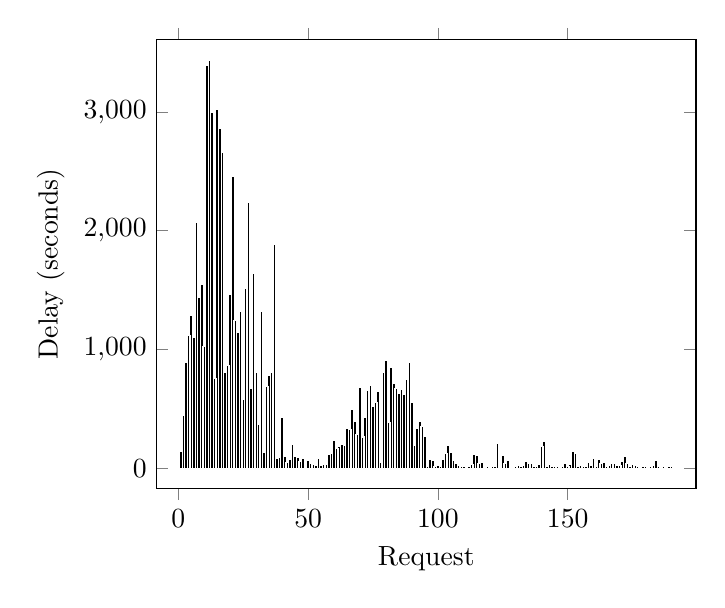
\begin{tikzpicture}
      \begin{axis}[
         ylabel=Delay (seconds),
         xlabel=Request,
         bar width=1pt,
         enlarge x limits=0.05,
         enlarge y limits=0.05,
         ybar
      ]
      \addplot+[draw=white, fill=black] coordinates
      {(1, 140) (2, 449) (3, 888) (4, 1119) (5, 1283) (6, 1099) (7, 2071) (8, 1439) (9, 1550) (10, 1023) (11, 3393) (12, 3435) (13, 2991) (14, 758) (15, 3021) (16, 2858) (17, 2658) (18, 808) (19, 865) (20, 1461) (21, 2459) (22, 1244) (23, 1144) (24, 1321) (25, 584) (26, 1513) (27, 2240) (28, 670) (29, 1644) (30, 810) (31, 374) (32, 1317) (33, 134) (34, 688) (35, 785) (36, 809) (37, 1881) (38, 86) (39, 93) (40, 428) (41, 104) (42, 46) (43, 78) (44, 201) (45, 97) (46, 96) (47, 61) (48, 80) (49, 8) (50, 66) (51, 43) (52, 31) (53, 27) (54, 83) (55, 28) (56, 36) (57, 32) (58, 116) (59, 126) (60, 233) (61, 165) (62, 186) (63, 205) (64, 190) (65, 340) (66, 327) (67, 495) (68, 398) (69, 282) (70, 680) (71, 264) (72, 428) (73, 654) (74, 696) (75, 519) (76, 555) (77, 649) (78, 52) (79, 811) (80, 909) (81, 387) (82, 848) (83, 712) (84, 673) (85, 628) (86, 661) (87, 623) (88, 746) (89, 889) (90, 552) (91, 194) (92, 335) (93, 398) (94, 350) (95, 267) (96, 20) (97, 78) (98, 70) (99, 15) (100, 22) (101, 15) (102, 73) (103, 129) (104, 191) (105, 137) (106, 71) (107, 39) (108, 26) (109, 14) (110, 13) (111, 11) (112, 18) (113, 32) (114, 117) (115, 113) (116, 42) (117, 49) (118, 9) (119, 13) (120, 6) (121, 19) (122, 16) (123, 207) (124, 12) (125, 110) (126, 42) (127, 70) (128, 11) (129, 12) (130, 15) (131, 23) (132, 17) (133, 21) (134, 62) (135, 44) (136, 40) (137, 13) (138, 19) (139, 32) (140, 188) (141, 225) (142, 13) (143, 31) (144, 19) (145, 15) (146, 19) (147, 11) (148, 18) (149, 38) (150, 16) (151, 33) (152, 139) (153, 130) (154, 16) (155, 26) (156, 14) (157, 20) (158, 52) (159, 24) (160, 87) (161, 20) (162, 75) (163, 43) (164, 53) (165, 16) (166, 23) (167, 41) (168, 45) (169, 21) (170, 24) (171, 58) (172, 98) (173, 38) (174, 20) (175, 33) (176, 28) (177, 19) (178, 12) (179, 15) (180, 15) (181, 8) (182, 13) (183, 24) (184, 64) (185, 15) (186, 10) (187, 13) (188, 8) (189, 15) (190, 13)};
   \end{axis}
\end{tikzpicture}
   \caption{this is the caption}
   
\end{figure*}
\section*{Solution}

\def\arraystretch{1.5}
\begin{table*}[ht]
\small
   \centering
   \begin{tabular}{ l | c | c | c | c | c }
      \textit& Monday & Tuesday & Wednesday & Thursday & Friday \\ \hline
      12:30 & 51, 65, 66 & 16, 19, 45, 46, 61 & 24, 40, 43, 50 & 5, 15, 39 & 6, 25, 27 \\
      1:30 & 54, 60, 65, 66 & 16, 19, 20, 34, 61 & 24, 40, 44, 63 & 5, 12, 22, 64 & 1, 25, 27 \\
      2:30 & 42, 51, 52, 54, 60 & 16, 20, 34, 55, 57, 61 & 7, 24, 44, 50, 63 & 5, 12, 13, 22, 33, 64 & 3, 4, 6, 9, 47 \\
      3:30 & 32, 37, 38, 42, 45, 46 & 16, 18, 20, 49, 55, 57, 61 & 7, 36, 40, 44, 58, 63 & 11, 12, 22, 33, 59 & 1, 25, 27, 47, 53 \\
      4:30 & 30, 32, 37, 38, 39, 41 & 16, 18, 20, 34, 49 & 24, 36, 41, 43, 44, 58 & 5, 11, 12, 13, 33, 59, 64 & 1, 3, 6, 25, 53 \\
      5:30 & 23, 26, 28, 29, 30 & 34, 55 & 24, 36, 40, 44, 50, 63 & 5, 11, 13, 22, 33, 64 & 4, 6, 47, 53 \\
      6:30 & 17, 21, 23, 26, 28 & 18, 20, 34, 55, 57, 61 & 7, 36, 40, 58, 63 & 5, 12, 13, 22, 33, 64 &  \\
      7:30 & 10, 14, 17, 21 & 18, 20, 34, 55, 57 & 7, 24, 36, 40, 58 & 5, 12, 13, 22, 33, 64 &  \\
      8:30 & 9, 10, 14, 15 & 18, 20, 34, 55, 57 & 7, 36, 44, 58 & 5, 12, 13, 22, 33 &  \\
   \end{tabular}
   \\[10pt]
   \centering
   \begin{tabular}{ l | c | c }   
      \textit & Saturday & Sunday \\ \hline
      1:30 & 35, 52, 62 & 0, 8, 31 \\
      2:30 & 2, 35, 48 & 0, 8, 31 \\
      3:30 & 2, 29, 35, 48 & 0, 8, 31, 56 \\
      4:30 & 2, 35, 48, 62 & 0, 8, 31, 56 \\
   \end{tabular}
   \\[10pt]
   \caption*{Time slot assignments for the sixty-seven TAs working during Autumn 2014. Each cell contains the TAs assigned to a given hour on a given day.}
\end{table*}
\end{multicols}
\end{document}
